\documentclass[a4paper,14pt]{article}

\usepackage{comment} % Para comentar várias linhas ao mesmo tempo

%matemática
\usepackage{amsmath}
\usepackage{amssymb}

%diagramação
\usepackage{extsizes}
\everymath{\displaystyle}
\usepackage{geometry}
\usepackage{fancyhdr}
\usepackage{multicol}
\usepackage{graphicx}
\usepackage[brazil]{babel}
\usepackage[shortlabels]{enumitem}
\usepackage{cancel}
\usepackage{textcomp}
\usepackage{tcolorbox}

%tabelas
\usepackage{array} % Para melhor formatação de tabelas
\usepackage{longtable}
\usepackage{booktabs}  % Para linhas horizontais mais bonitas
\usepackage{float}   % Para usar o modificador [H]
\usepackage{caption} % Para usar legendas em tabelas
\usepackage{wrapfig} % Para usar tabelas e figuras flutuantes
\usepackage{xcolor} % Para cores do fundo de tabelas
\usepackage{colortbl} % Para cores do fundo de tabelas

%tikzpicture
\begin{comment}
	\usepackage{tikz}
	\usepackage{scalerel}
	\usepackage{pict2e}
	\usepackage{tkz-euclide}
	\usetikzlibrary{calc}
	\usetikzlibrary{patterns,arrows.meta}
	\usetikzlibrary{shadows}
	\usetikzlibrary{external}
\end{comment}


%pgfplots
\usepackage{pgfplots}
\pgfplotsset{compat=newest}
\usepgfplotslibrary{statistics}
\usepgfplotslibrary{fillbetween}

%colours
\usepackage{xcolor}



\columnsep=2cm
\hoffset=0cm
\textwidth=8cm
\setlength{\columnseprule}{.1pt}
\setlength{\columnsep}{2cm}
\renewcommand{\headrulewidth}{0pt}
\geometry{top=1in, bottom=1in, left=0.7in, right=0.5in}

\pagestyle{fancy}
\fancyhf{}
\fancyfoot[C]{\thepage}

\begin{document}
	
	\noindent\textbf{6FMA22 - Matemática} 
	
	\begin{center}Oposto de um número inteiro (Versão estudante)
	\end{center}
	
	\noindent\textbf{Nome:} \underline{\hspace{10cm}}
	\noindent\textbf{Data:} \underline{\hspace{4cm}}
	
	%\section*{Questões de Matemática}
	
	\begin{multicols}{2}
		\noindent O oposto (ou simétrico) de um número inteiro $x$ é o número que está à mesma distância de $x$ ao zero, mas em sentido oposto. Indicamos o oposto de $x$ por $-x$ e lemos: oposto de $x$ ou simétrico de $x$ ou menos $x$. O oposto de zero é zero e o oposto do oposto de $x$ é o próprio $x$, isto é, $-(-x) = x$ \\
		\noindent\textsubscript{-----------------------------------------------------------------------}
		\begin{enumerate} 
			\item Escreva usando símbolos:
			\begin{enumerate}[a)] 
				\item o oposto de 5. \\\\\\
				\item o simétrico de -3. \\\\\\
				\item o oposto do oposto de -4. \\\\\\
			\end{enumerate}
			\item Complete:
			\begin{enumerate}[a)] 
				\item O oposto de 7 é $\underline{~~~~~~}$. \\
				\item O oposto de -1 é $\underline{~~~~~~}$. \\
				\item -(-5) = $\underline{~~~~~~}$. \\
				\item O oposto do oposto de -(-2) é $\underline{~~~~~~}$. \\ 
				\item -(-(-4)) = $\underline{~~~~~~}$. \\
			\end{enumerate}
			\item Em cada item, observe a ilustração e o sentido da reta e escreva o que se pede.
			\begin{enumerate}[a)] 
				\item ~ \\ 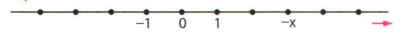
\includegraphics[width=1.1\linewidth]{6FMA22_imagens/imagem1} \\
				$x = \underline{~~~~~~} ~~~~~~~~ -x = \underline{~~~~~~}$ \\
				$x$ é positivo, negativo ou nulo? \\\\\\\\
				$-x$ é positivo, negativo ou nulo? \\\\\\\\
				\item ~ \\ 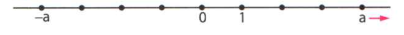
\includegraphics[width=1.1\linewidth]{6FMA22_imagens/imagem2} \\
				$a = \underline{~~~~~~} ~~~~~~~~ -a = \underline{~~~~~~}$ \\
				$a$ é positivo, negativo ou nulo? \\\\\\\\
				$-a$ é positivo, negativo ou nulo? \\
				\item ~ \\ 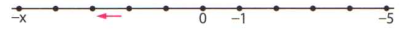
\includegraphics[width=1.1\linewidth]{6FMA22_imagens/imagem3} \\
				$x = \underline{~~~~~~} ~~~~~~~~ -x = \underline{~~~~~~}$ \\
				$x$ é positivo, negativo ou nulo? \\\\\\\\
				$-x$ é positivo, negativo ou nulo? \\\\\\\\
				\item ~ \\ 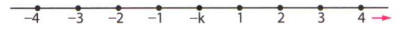
\includegraphics[width=1.1\linewidth]{6FMA22_imagens/imagem4} \\
				$k = \underline{~~~~~~} ~~~~~~~~ -k = \underline{~~~~~~}$ \\
				$k$ é positivo, negativo ou nulo? \\\\\\\\
				$-k$ é positivo, negativo ou nulo? \\\\\\\\
			\end{enumerate}
			\item Veja as ilustrações a seguir e escreva quanto vale $x$ e quanto vale $-x$. Observe a orientação das retas.
			\begin{enumerate}[a)] 
				\item ~ \\ 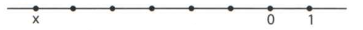
\includegraphics[width=1.1\linewidth]{6FMA22_imagens/imagem5} \\\\\\
				\item ~ \\
				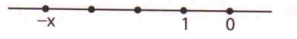
\includegraphics[width=1.1\linewidth]{6FMA22_imagens/imagem6} \\\\\\
				\item ~ \\
				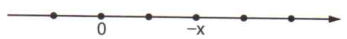
\includegraphics[width=1.1\linewidth]{6FMA22_imagens/imagem7} \\\\\\
				\item ~ \\
				
\includegraphics[width=1.1\linewidth]{6FMA22_imagens/imagem8} \\\\\\
			\end{enumerate}
			\item Complete:
			\begin{enumerate}[a)] 
				\item Se $a = -5$, então $-a = \underline{~~~~~~}$. \\
				\item Se $-b = -6$, então $b = \underline{~~~~~~}$. \\
				\item Se $-c = 0$, então $c = \underline{~~~~~~}$. \\
				\item Se $d = 8$, então $-d = \underline{~~~~~~}$. \\
				\item Se $e = -2 001$, \\ então $-e = \underline{~~~~~~}$. 
			\end{enumerate}
			%76 a 80
			\item Assinale \textbf{V} (verdadeiro) ou \textbf{F} (falso).
			\begin{enumerate}[a)] 
				\item (~~) Se $x$ é inteiro, então $x$ é positivo.
				\item (~~) Se $x$ é inteiro, então $-x$ é negativo.
				\item (~~) Se $x$ é inteiro e $x > 0$, então $x$ é positivo.
				\item (~~) Se $x$ é inteiro e $x > 0$, então $-x$ é negativo.
				\item (~~) Se $x \in \mathbb{Z}$ e $x < 0$, então $x$ é positivo.
				\item (~~) Se $x \in \mathbb{Z}$ e $x < 0$, então $x$ é negativo.
				\item (~~) Se $x$ é inteiro e $x > 0$, então $-x$ é positivo.
				\item (~~) Se $x \in \mathbb{Z}$ e $x < 0$, então $-x$ é positivo.
				\item (~~) Se $x \in \mathbb{Z}$ e $-x$ é negativo, então $x$ é positivo.
				\item (~~) Para todo inteiro $x, -(-x) = x$.
			\end{enumerate}
			\item Assinale \textbf{V} (verdadeiro) ou \textbf{F} (falso).
			\begin{enumerate}[a)] 
				\item (~~) 3 = -(-3).
				\item (~~) O oposto de 5 é -(-5).
				\item (~~) 0 = -0.
				\item (~~) -(-(-7)) = -7.
				\item (~~) Todo número inteiro é diferente do seu oposto.
				\item (~~) Se $x$ é um número inteiro, então $-x$ também é inteiro.
				\item (~~) O simétrico do simétrico de -8 é -8.
				\item (~~) O oposto do oposto de 6 é -6.
			\end{enumerate}
			\item Complete.
			\begin{enumerate}[a)] 
				\item -(-7) = ..... .
				\item -(-(-6)) = ..... .
				\item 4 = ..... .
				\item -(-x) = ..... .
				\item x = -..... .
				\item -(-(-(-x))) = ..... .
				\item Se $-x > 0$, então $x$ ..... .
				\item Se $-x < 0$, então $x$ ..... .
			\end{enumerate}
			\item Dado $n \in \mathbb{Z}$:
			\begin{enumerate}[a)] 
				\item quando $-n$ é negativo? \\\\\\\\
				\item quando $-n$ é nulo? \\\\\\\\
				\item quando $-n$ é positivo? \\\\\\\\
			\end{enumerate}
			\item Complete.
			\begin{enumerate}[a)] 
				\item -(-1) = ..... .
				\item -(-(-5)) = ..... .
				\item Se $x > 0$, então $-x$ ..... 0.
				\item Se $-x < 0$, então $x$ ..... 0.
				\item Se $x < 0$, então $-x$ ..... 0.
				\item Se $-x > 0$, então $x$ ..... 0.
			\end{enumerate}
		\end{enumerate}
		$~$ \\ $~$ \\ $~$ \\ $~$ \\ $~$ \\ $~$ \\ $~$ \\ $~$ \\ $~$ \\
	\end{multicols}
\end{document}